% SIMULATION ARCHITECTURE
% Last generated: 2026-01-15T05:34:34.872Z

\subsection{System Overview}

Our simulation framework consists of four main components (Figure~\ref{fig:architecture}):

\begin{enumerate}
    \item \textbf{Configuration Layer}: YAML/JSON experiment definitions
    \item \textbf{Simulation Engine}: Core DAO state machine and agent behaviors
    \item \textbf{Batch Runner}: Concurrent execution with checkpoint/resume
    \item \textbf{Analysis Pipeline}: Export to CSV/JSON for statistical analysis
\end{enumerate}

\begin{figure}[htbp]
    \centering
    % AUTO-GENERATED: architecture diagram
    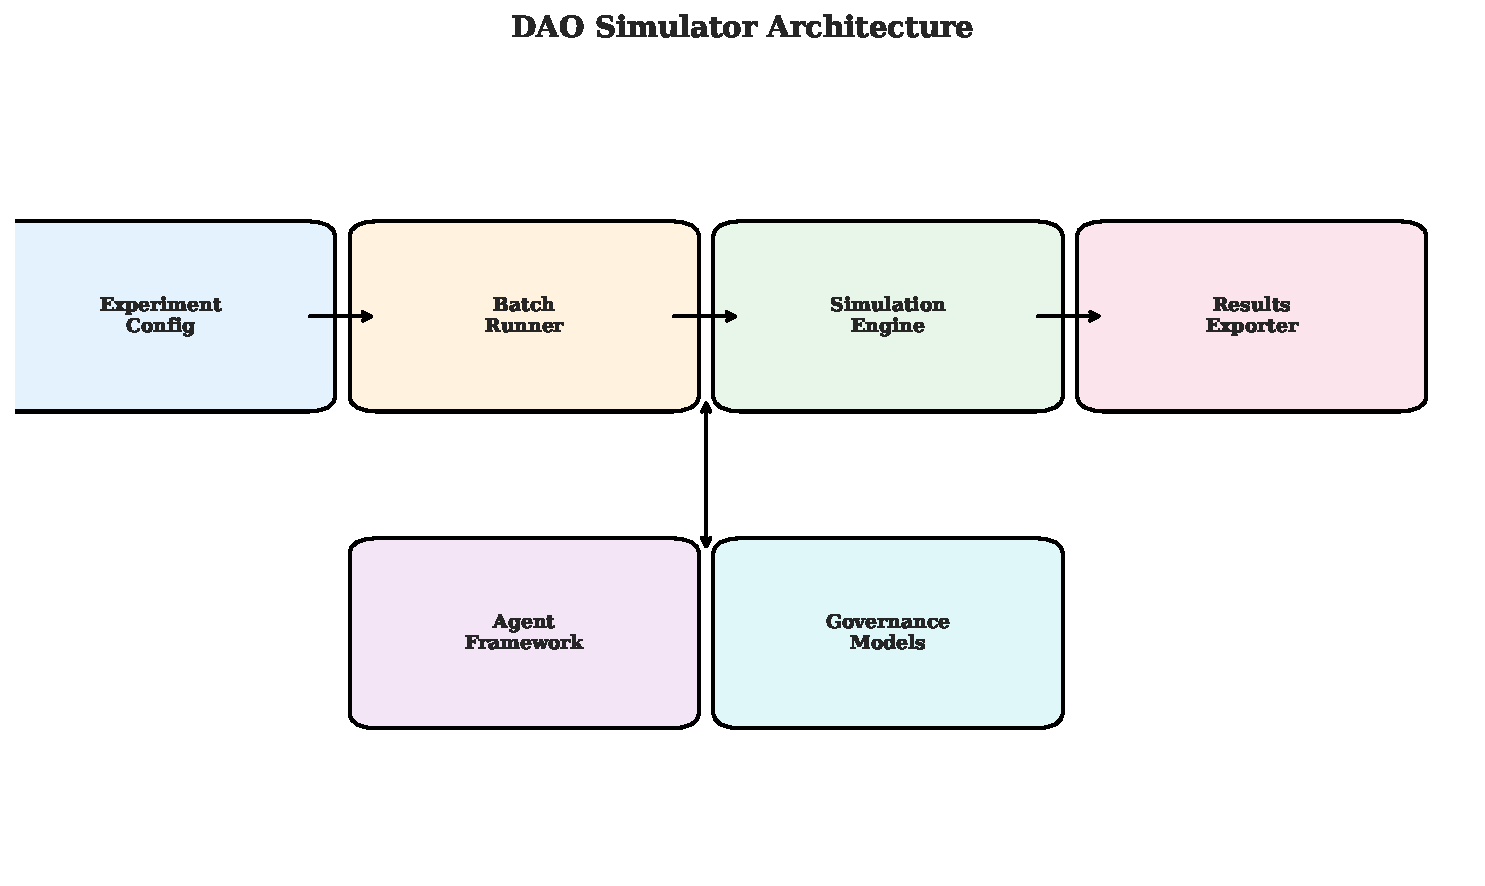
\includegraphics[width=0.8\textwidth]{figures/architecture}
    \caption{Simulation framework architecture. The configuration layer accepts experiment definitions. The engine executes simulations with multiple voting mechanisms. Results are exported for statistical analysis.}
    \label{fig:architecture}
\end{figure}

\subsection{Agent Implementation}

Agents are implemented as autonomous decision-makers with:

\begin{lstlisting}[language=Python, caption=Agent behavior model (pseudocode)]
class Agent:
    def decide_participation(self, proposal):
        if self.delegation_target:
            return DELEGATE

        relevance = self.compute_relevance(proposal)
        cost = self.attention_cost

        if relevance > cost * self.threshold:
            return VOTE
        return ABSTAIN

    def compute_vote(self, proposal):
        alignment = dot(self.preferences, proposal.impact)
        return SUPPORT if alignment > 0 else OPPOSE
\end{lstlisting}

\subsubsection{Agent Types}

The framework supports heterogeneous agent populations:

\begin{table}[htbp]
\centering
\caption{Agent archetypes and their behavioral parameters}
\label{tab:agent-types}
\begin{tabular}{lcccc}
\toprule
Type & Participation & Token Share & Delegation & Description \\
\midrule
Whale & 0.8 & 20-30\% & Self & Large holders, high engagement \\
Delegate & 0.9 & 5-10\% & Self & Professional governance \\
Active & 0.5 & 30-40\% & Variable & Regular participants \\
Passive & 0.1 & 20-30\% & Often & Occasional voters \\
\bottomrule
\end{tabular}
\end{table}

\subsection{Governance Mechanisms}

\subsubsection{Voting Systems}

The framework implements multiple voting mechanisms:

\begin{itemize}
    \item \textbf{Token Voting}: Standard 1-token-1-vote with delegation
    \item \textbf{Quadratic Voting}: Square root of tokens determines weight
    \item \textbf{Conviction Voting}: Time-weighted voting with decay
    \item \textbf{Approval Voting}: Continuous approval for executives
\end{itemize}

\subsubsection{Quorum Mechanisms}

Supported quorum types:
\begin{itemize}
    \item \textbf{Fixed Percentage}: Constant threshold (e.g., 4\%)
    \item \textbf{Dynamic}: Adjusts based on recent participation
    \item \textbf{Per-Category}: Different thresholds for proposal types
\end{itemize}

\subsection{Simulation Loop}

Each simulation step represents one day:

\begin{algorithmic}
\FOR{step = 1 to max\_steps}
    \STATE Generate new proposals based on frequency
    \STATE Update proposal states (advance stages)
    \FOR{each active proposal}
        \FOR{each agent}
            \STATE Agent decides: vote, delegate, or abstain
        \ENDFOR
        \STATE Tally votes, check quorum
    \ENDFOR
    \STATE Execute passed proposals
    \STATE Update treasury, token distributions
    \STATE Collect metrics
\ENDFOR
\end{algorithmic}

\subsection{Reproducibility Features}

The framework ensures reproducibility through:

\begin{itemize}
    \item \textbf{Deterministic Seeding}: All random operations use seeded PRNGs
    \item \textbf{Configuration Hashing}: Experiments are identified by config hash
    \item \textbf{Manifests}: Each run produces a reproducibility manifest with:
        \begin{itemize}
            \item Git commit hash
            \item Node.js version
            \item All random seeds used
            \item Results hash for verification
        \end{itemize}
\end{itemize}

\subsection{Implementation}

The framework is implemented in TypeScript, chosen for:
\begin{itemize}
    \item Type safety reducing runtime errors
    \item Async/await for concurrent execution
    \item NPM ecosystem for data processing
    \item Web interface integration (Designer UI)
\end{itemize}

Total implementation: approximately 5,000 lines of code across simulation engine, research CLI, and visualization components.
